%%%%%%%%%%%%%%%%%%%%%%%%%%%%%%%%%%%%%%%%%%%%%%%%%%%%
%%%%%%% Verslag Tinlab Advanced Algoritms %%%%%%%
%%%%%%%%%%%%%%%%%%%%%%%%%%%%%%%%%%%%%%%%%%%%%%%%%%%%

\documentclass{article}
\usepackage{graphicx}
\usepackage[font=small,labelfont=bf]{caption}
\usepackage[dutch]{babel}

\begin{document}

	\sffamily
	%%%%%%% Front page %%%%%%%
	%%%%%%%%%%%%%%%%%%%%%%%%%%%%%%%%%%%%%%%%%%%%%%%%%%%%
	
	\begin{titlepage}
	
		\centering
		  \vfill
		  {\bfseries\Huge
		    Verslag Tinlab Advanced Algorithms \\
		      \vskip2cm
		    }
		    {\bfseries\Large
		      Thijs Dregmans\\
		    }
		    {
		      \bfseries\normalsize
		      1024272\\
		      \vskip1cm
		      \today\\
		  }    
		  \vfill
		  
\includegraphics[width=4cm]{logohr.png} % also works with logo.pdf
		  \vfill
		  \vfill
	    
	\end{titlepage}
	
	\newpage
	
	%%%%%%% Table of Content %%%%%%%
	%%%%%%%%%%%%%%%%%%%%%%%%%%%%%%%%%%%%%%%%%%%%%%%%%%%%
	
	\tableofcontents
	
	\newpage
	
	%%%%%%% Inleiding %%%%%%%
	%%%%%%%%%%%%%%%%%%%%%%%%%%%%%%%%%%%%%%%%%%%%%%%%%%%%
	
	\section{Inleiding}
	
	Voor de cursus 'Advanced Algorithms' van de opleiding Technische Informatica heb ik het volgende verslag geschreven. Het is een verwerking en samenvatting van de lesstof. Het dient zowel als naslagwerk voor mijzelf, als het aantonen van het behalen van de leerdoelen voor de cursus.
	
	Het Tinlab begon met het behandelen van het probleem van specificeren van requirements. Dit is alle design domeinen een groot probleem. Goede requirements definieren is een hoofdpijn dossier. We hebben naar systemen gekeken door het vier variabelen model. Vervolgens zijn een aantal rampen bekeken om dit model in de praktijk te gebruiken om uitspraken te doen over het falen van systemen.

	[geef een samenvatting van de cursus]
	
	\newpage
	
	%%%%%%% Requirements %%%%%%%
	%%%%%%%%%%%%%%%%%%%%%%%%%%%%%%%%%%%%%%%%%%%%%%%%%%%%
	
	\section{Requirements}
	
		Requirements zijn eisen die gesteld worden aan een systeem.

		[aanvullen]
		
		%%%%%%%%%%%%%%%%%%%%%%%%%%%%%%%%%%%%%%%%%%%%%%%%%%%%
		\subsection{Requirements}
		
		[text]
		
		%%%%%%%%%%%%%%%%%%%%%%%%%%%%%%%%%%%%%%%%%%%%%%%%%%%%
		\subsection{specificaties}
		
		[text]
		
		%%%%%%%%%%%%%%%%%%%%%%%%%%%%%%%%%%%%%%%%%%%%%%%%%%%%
		\subsection{Het vier variabelen model}
		
		Een handige manier om systemen te conceptualiseren is het vier variabelen model. Zie Figuur 1 voor een uitwerking van dit model.
		
		\begin{center}
			\begin{minipage}{0.48\linewidth}
				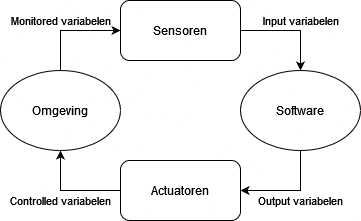
\includegraphics[width=\linewidth]{4variabelen.png}
				\captionof{figure}{4 variabelen model}
			\end{minipage}
			\hfill
		\end{center}

		Dit model komt vooruit het idee van twee werelden die overlappen. Er is een tastbare wereld, met verschillende fenomenen. Deze wereld is de werld waarin wij leven. In deze wereld zijn problemen die wij willen oplossen met systemen. Zo'n systeem is geen onderdeel van de tastbare wereld. Het systeem is een wereld op zichzelf. Er wel enig overlap tussen de syteem-wereld en de tastbare wereld. Het overlap tussen deze werelden is de hardware, specifiek de sensoren en actuatoren.

		De systeem-wereld is de software. Deze wereld heeft in zichzelf geen enkel idee van het bestaan van een ander wereld. De tastbare wereld is de omgeving waarin de het systeem functioneert (of moet functioneren). Ook deze wereld heeft geen idee van de werking van de ander. Dit is ook niet mogelijk of belangrijk, zolang de sensoren en actuatoren naar behoren functioneren.

		De 4 verschillende delen van de van de werelden - omgeving, sensoren, software en actuatoren - communiceren met elkaar met behulp van variabelen.
		
			%%%%%%%%%%%%%%%%%%%%%%%%%%%%%%%%%%%%%%%%%%%%%%%%%%%%
			\subsubsection{Monitored variabelen}
			
			Monitored variabelen zijn de variabelen uit de wereld die door de sensoren wordt waargenomen en gemeten.
			
			Ter voorbeeld, een Monitored variabele kan de temperatuur zijn. De omgeving is bijvoorbeeld binnenshuis, bij iemand thuis. De sensor is een temperatuursensor. De sensor meet de waarde/variabele.
			
			%%%%%%%%%%%%%%%%%%%%%%%%%%%%%%%%%%%%%%%%%%%%%%%%%%%%
			\subsubsection{Input variabelen}
			
			Input variabelen zijn de variabelen die door de sensor worden doorgegeven aan de software.

			In het voorbeeld van de temperatuursensor, heeft de temperatuursensor de Monitored variabele omgezet in een reeks bits. Deze bits worden door de sensor naar de microcontroller gestuurd. Voor de software die op de microcontroller staat, is dit de input. In het syteem geldt deze bits als Input variabele.
			
			%%%%%%%%%%%%%%%%%%%%%%%%%%%%%%%%%%%%%%%%%%%%%%%%%%%%
			\subsubsection{Output variabelen}
			
			Output variabelen zijn de variabelen die door de software worden geproduceerd en worden doorgegeven aan de actuatoren.

			In het voorbeeld, heeft de software van de microcontroller de temperatuur - in de vorm van een aantal bits - omgezet in een output. De output is in dit voorbeeld een instructie voor een warmte element om aan te gaan, indien de temperatuur onder een bepaalde waarde zakt. De instructie voor het warmte element is de output van de software, en daarom - in dit voorbeeld - de Output variabele.

			%%%%%%%%%%%%%%%%%%%%%%%%%%%%%%%%%%%%%%%%%%%%%%%%%%%%
			\subsubsection{Controlled variabelen}

			Controlled variabelen zijn de variabelen in de omgeving die door de actuatoren worden beïnvloed, of 'Controlled'.

			In dit voorbeeld, is er door de microcontroller een instructie gegeven aan het warmte element. De microcontroller bevat de software en het warmte element is de actuator. Door de instructie van de software gaat het warmte element aan, en wordt het warmer in huis. De temperatuur stijgt. De Controlled variabele in dit voorbeeld is de temperatuur.

			
			In dit voorbeeld is de Controlled variabele en de Monitored variabele dezelfde variabele, maar dat hoeft niet zo te zijn. Men kan in plaats van een warmte element, ook een lampje aansluiten, die dan aan zou gaan bij een bepaalde temperatuur. In dit geval zou de Controlled variabele het licht van het lampje zijn.
		
		%%%%%%%%%%%%%%%%%%%%%%%%%%%%%%%%%%%%%%%%%%%%%%%%%%%%
		\subsection{Rampen}
		
		De werking van het vier variabelen model wordt gedemonstreerd aan de hand van een aantal verschillende rampen.
		
			%%%%%%%%%%%%%%%%%%%%%%%%%%%%%%%%%%%%%%%%%%%%%%%%%%%%
			\subsubsection{Ramp 1}
			\begin{description}
			\item[Beschrijving]
			\item[Datum en plaats] 
			\item[Oorzaak]
			  %Beschrijf wat er mis ging in termen van het vier variabelen model/requirements/specificaties
			\end{description}
			
			%%%%%%%%%%%%%%%%%%%%%%%%%%%%%%%%%%%%%%%%%%%%%%%%%%%%
			\subsubsection{Ramp 2}
			\begin{description}
			\item[Beschrijving]
			\item[Datum en plaats] 
			\item[Oorzaak]
			  %Beschrijf wat er mis ging in termen van het vier variabelen model/requirements/specificaties
			\end{description}
			
			%%%%%%%%%%%%%%%%%%%%%%%%%%%%%%%%%%%%%%%%%%%%%%%%%%%%
			\subsubsection{Ramp 3}
			\begin{description}
			\item[Beschrijving]
			\item[Datum en plaats] 
			\item[Oorzaak]
			  %Beschrijf wat er mis ging in termen van het vier variabelen model/requirements/specificaties
			\end{description}
			
			%%%%%%%%%%%%%%%%%%%%%%%%%%%%%%%%%%%%%%%%%%%%%%%%%%%%
			\subsubsection{Ramp 4}
			%%%%%%%%%%%%%%%%%%%%%%%%%%%%%%%%%%%%%%%%%%%%%%%%%%%%
			\subsubsection{Ramp 5}
			%%%%%%%%%%%%%%%%%%%%%%%%%%%%%%%%%%%%%%%%%%%%%%%%%%%%
			\subsubsection{Ramp 6}
		
	\newpage
	
	%%%%%%% Modellen %%%%%%%
	%%%%%%%%%%%%%%%%%%%%%%%%%%%%%%%%%%%%%%%%%%%%%%%%%%%%
	
	\section{Modellen}
	
	[text]
	
		%%%%%%%%%%%%%%%%%%%%%%%%%%%%%%%%%%%%%%%%%%%%%%%%%%%%
		\subsection{De Kripke structuur}
		
		[text]
		
		%%%%%%%%%%%%%%%%%%%%%%%%%%%%%%%%%%%%%%%%%%%%%%%%%%%%
		\subsection{Soorten modellen}
		
		\newpage
		
		%%%%%%%%%%%%%%%%%%%%%%%%%%%%%%%%%%%%%%%%%%%%%%%%%%%%
		\subsection{Tijd}
		
		[text]
		
		%%%%%%%%%%%%%%%%%%%%%%%%%%%%%%%%%%%%%%%%%%%%%%%%%%%%
		\subsection{Guards en invarianten}
		
		[text]
		
		%%%%%%%%%%%%%%%%%%%%%%%%%%%%%%%%%%%%%%%%%%%%%%%%%%%%
		\subsection{Deadlock}
		
		[text]
		
		%%%%%%%%%%%%%%%%%%%%%%%%%%%%%%%%%%%%%%%%%%%%%%%%%%%%
		\subsection{Zeno gedrag}
		
		[text]
		
	\newpage
	
	%%%%%%% Logica %%%%%%%
	%%%%%%%%%%%%%%%%%%%%%%%%%%%%%%%%%%%%%%%%%%%%%%%%%%%%
	
	\section{Logica}
	
	[text]
	
		%%%%%%%%%%%%%%%%%%%%%%%%%%%%%%%%%%%%%%%%%%%%%%%%%%%%
		\subsection{Propositielogica}
		
		[text]
		
		%%%%%%%%%%%%%%%%%%%%%%%%%%%%%%%%%%%%%%%%%%%%%%%%%%%%
		\subsection{Predicatenlogica}
		
		[text]
		
		%%%%%%%%%%%%%%%%%%%%%%%%%%%%%%%%%%%%%%%%%%%%%%%%%%%%
		\subsection{Kwantoren}
		
		[text]
		
		%%%%%%%%%%%%%%%%%%%%%%%%%%%%%%%%%%%%%%%%%%%%%%%%%%%%
		\subsection{Dualiteiten}
		
		[text]
	
	\newpage
	
	%%%%%%% tree logic %%%%%%%
	%%%%%%%%%%%%%%%%%%%%%%%%%%%%%%%%%%%%%%%%%%%%%%%%%%%%
	
	\section{Computation tree logic}
	
	[text]
		
		%%%%%%%%%%%%%%%%%%%%%%%%%%%%%%%%%%%%%%%%%%%%%%%%%%%%
		\subsection{De computation tree}
				
		[text]
		
		%%%%%%%%%%%%%%%%%%%%%%%%%%%%%%%%%%%%%%%%%%%%%%%%%%%%
		\subsection{Operator: AG}
				
		[text]
		
		%%%%%%%%%%%%%%%%%%%%%%%%%%%%%%%%%%%%%%%%%%%%%%%%%%%%
		\subsection{Operator: EG}
				
		[text]
		
		%%%%%%%%%%%%%%%%%%%%%%%%%%%%%%%%%%%%%%%%%%%%%%%%%%%%
		\subsection{Operator: AF}
				
		[text]
		
		%%%%%%%%%%%%%%%%%%%%%%%%%%%%%%%%%%%%%%%%%%%%%%%%%%%%
		\subsection{Operator: EF}
				
		[text]
		
		%%%%%%%%%%%%%%%%%%%%%%%%%%%%%%%%%%%%%%%%%%%%%%%%%%%%
		\subsection{Operator: AX}
				
		[text]
		
		%%%%%%%%%%%%%%%%%%%%%%%%%%%%%%%%%%%%%%%%%%%%%%%%%%%%
		\subsection{Operator: EX}
				
		[text]
		
		%%%%%%%%%%%%%%%%%%%%%%%%%%%%%%%%%%%%%%%%%%%%%%%%%%%%
		\subsection{Operator: p U q}
				
		[text]
		
		%%%%%%%%%%%%%%%%%%%%%%%%%%%%%%%%%%%%%%%%%%%%%%%%%%%%
		\subsection{Operator: p R q}
				
		[text]
		
		%%%%%%%%%%%%%%%%%%%%%%%%%%%%%%%%%%%%%%%%%%%%%%%%%%%%
		\subsection{Fairness}
				
		[text]
		
		%%%%%%%%%%%%%%%%%%%%%%%%%%%%%%%%%%%%%%%%%%%%%%%%%%%%
		\subsection{Liveness}
			
		[text]
		
		%%%%%%%%%%%%%%%%%%%%%%%%%%%%%%%%%%%%%%%%%%%%%%%%%%%%
	
	\newpage
	
	%%%%%%% references %%%%%%%
	%%%%%%%%%%%%%%%%%%%%%%%%%%%%%%%%%%%%%%%%%%%%%%%%%%%%
	
	\bibliography{references}
	\bibliographystyle{plain}
	
\end{document}


